\documentclass{article}
\usepackage{amsmath}
\usepackage{amssymb}
\usepackage{graphicx}
\topmargin=-1in
\evensidemargin=0in
\oddsidemargin=0in
\textwidth=6.5in
\textheight=9.0in
\headsep=0.25in


\begin{document}
\title{\textbf {Hoja de Trabajo No. 2}}
\author{Sebastian Gomez}
\maketitle

\begin{center}
\textbf{EJERCICIO NO. 1}
\end{center}

En base a la ecuación 

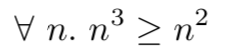
\includegraphics {EJERCICIO1T2.png}
\begin{itemize}
\item Paso Base
\item n = 0
\item $0^3\geq 0^2$
\item $0 \geq 0$
\item Paso de Inducción 
\item n = n + 1
\item $(n + 1)^3 \geq (n+1)^2$
\item $(n + 1)^3/(n + 1)^2 \geq 1$
\item $(n + 1) = 1$
\item $(n + 1) - 1 \geq 1 - 1$
\item $n \geq 0$
\end{itemize}

\begin{center}
\textbf {EJERCICIO NO. 2}
\end{center}
\begin{itemize}
\item Paso Base
\item Para n = 0, y x $\geq$ - 1 
\item $(1 + x)^0 \geq 1 + 0x$ 
\item 1 = 1 + 0
\item Paso Inducción
\item n = n + 1
\item Se multiplica por (1 + x) en ambos lados de la función, porque $x \geq -1$ es igual a $1 + x \geq 0$ 
\item $(1 + x)^{n+1} \geq (1 + nx)(1+x)$
\item $(1 + x)^{n+1} \geq 1 + (n + 1)x + nx^2$
\item Ya que $nx^2 \geq 0$, se evalua para (n + 1) la siguiente función $(1 + x)^{n+1} \geq 1 + (n + 1)x$
\item Para n = 1 y para x $\geq$ 1
\item $(1 - 1)^{1+1}\geq 1 + (1 + 1)(-1)$
\item $0 \geq -2$
\end{itemize}



\end{document}
